\documentclass[letterpaper, 11pt]{article}
%\usepackage[round]{natbib}

\usepackage{placeins}
\usepackage{mathtools}
\usepackage{setspace} 
\usepackage{dsfont}
\usepackage{amsfonts}
\usepackage{amsmath}
\usepackage{subcaption}
\usepackage{paralist}
%\usepackage{subfig}
\usepackage{times}
\usepackage{latexsym}
\usepackage{graphicx}
\usepackage[T1]{fontenc}
\usepackage{tikz}
\usepackage{url}
\usepackage{pgfplotstable}
\usepackage{titlesec}
\usepackage{color}
\usepackage{lipsum,adjustbox}
\usepackage[font={small}]{caption}
\usetikzlibrary{positioning}
\usepackage{bbm}
\usepackage{numprint}
\usepackage{booktabs}

\makeatletter
\newcommand{\@BIBLABEL}{\@emptybiblabel}
\newcommand{\@emptybiblabel}[1]{}
%\makeatother
\usepackage[draft,hidelinks]{hyperref}
\setlength{\parskip}{-.05em}

\usepackage{naaclhlt2018}
\graphicspath{{./plots/}}
\newcommand{\com}[1]{}
%\newcommand{\oa\part{title}}[1]{}
%\newcommand{\lc}[1]{}
%\newcommand{\oa}[1]{}
\newcommand{\oa}[1]{\footnote{\color{red}OA: #1}}
\newcommand{\oamod}[1]{{\color{red}#1}}
\newcommand{\lc}[1]{\footnote{\color{blue}LC: #1}}
\newcommand{\lcmod}[1]{{\color{blue}#1}}

\newenvironment{myequation}{
  \vspace{-1em}
 \begin{equation}
}{
 \end{equation}
 \vspace{-1.2em}
}
\newenvironment{myequation*}{
	\vspace{-1em}
	\begin{equation*}
}{
\end{equation*}
\vspace{-1.2em}
}
\begin{document}
\appendix

\title{}
%\maketitle

\onecolumn


\section{Systems tested}\label{ap:abbr}
Adam Mickiewicz University (AMU),
University of Cambridge (CAMB), Columbia University and the University of Illinois at Urbana-Champaign (CUUI),
Indian Institute of Technology, Bombay (IITB), Instituto Politecnico Nacional (IPN),
National Tsing Hua University (NTHU), Peking University (PKU), Pohang University of Science and Technology (POST),
Research Institute for Artificial Intelligence, Romanian Academy (RAC), Shanghai Jiao Tong University (SJTU),
University of Franche Comt\'{e} (UFC), University of Macau (UMC), \newcite[RoRo]{rozovskaya2016grammatical}, \newcite[JMGR]{junczysdowmunt-grundkiewicz:2016:EMNLP2016} \newcite[Char]{xie2016neural}.

\section*{\centering\Large Supplementary Material for ``Inherent Biases in Reference-based Evaluation for
Grammatical Error Correction''}


\section{Collected references}\label{ap:crowd}
\subsection{Grammatical Error Correction}
\begin{table}[]
	\centering
	\begin{tabular}{ll}
		\cline{1-1}
		\multicolumn{1}{|l|}{origin} & Other relatives may have the same possibilities to have such kind of disease .        \\ \hline
		1                            & It is possible other relatives may have the same kind of disease .                    \\
		2                            & It is possible that other relatives may have the same kind of disease .               \\
		3                            & It's also possible for other relatives to have the same kind of disease.              \\
		4                            & Other relatives may also be predisposed to the same kind of diseases.                 \\
		5                            & Other relatives may be at risk to have the same disease.                              \\
		6                            & Other relatives may have be prone to having such diseases.                            \\
		7                            & Other relatives may have similar possibilities to have the same disease.              \\
		8                            & Other relatives may have the possibility of having the same kind of disease.          \\
		9                            & Other relatives may have the possibility to have the same such disease .              \\
		10                           & Other relatives may have the same chance of contracting the same kind of disease.     \\
		11                           & Other relatives may have the same chance of having that kind of disease.              \\
		12                           & Other relatives may have the same chance of suffering such diseases.                  \\
		13                           & Other relatives may have the same chances of having the same kind of disease.         \\
		14                           & Other relatives may have the same chance to have the same disease.                    \\
		15                           & Other relatives may have the same likelihood of having such a disease.                \\
		16                           & Other relatives may have the same possibilities of having such a disease .            \\
		17                           & Other relatives may have the same possibilities of having such a disease .            \\
		18                           & Other relatives may have the same possibilities of having such a disease.             \\
		19                           & Other relatives may have the same possibilities of having that kind of disease.       \\
		20                           & Other relatives may have the same possibilities of having the same kind of disease.   \\
		21                           & Other relatives may have the same possibilities to develop such a disease.            \\
		22                           & Other relatives may have the same possibilities to have such a disease .              \\
		23                           & Other relatives may have the same possibilities to have such a kind of disease.       \\
		24                           & Other relatives may have the same possibilities to have such a kind of disease.       \\
		25                           & Other relatives may have the same possibilities to have such kinds of diseases.       \\
		26                           & Other relatives may have the same possibilities to have the same kind of disease .    \\
		27                           & Other relatives may have the same possibilities to have this kind of disease .        \\
		28                           & Other relatives may have the same possibilities to have this kind of disease.         \\
		29                           & Other relatives may have the same possibility of developing the same kind of disease. \\
		30                           & Other relatives may have the same possibility of having said disease.                 \\
		31                           & Other relatives may have the same possibility of having the disease.                  \\
		32                           & Other relatives may have the same possibility of having this kind of disease .        \\
		33                           & Other relatives may have the same possibility to have such a kind of disease .        \\
		34                           & Other relatives may have the same possibility to have such kind of a disease .        \\
		35                           & Other relatives may have the same possibility to have such kind of disease .          \\
		36                           & Other relatives may have the same possibility to have such kinds of disease .         \\
		37                           & Other relatives may have the same possibility to have such kinds of diseases.         \\
		38                           & Other relatives may have the same possibility to have the same kind of disease.       \\
		39                           & Other relatives may have the same probability of having this disease .                \\
		40                           & Other relatives may have the same probability to have the same kind of disease.       \\
		41                           & Other relatives may have the same risk for developing such a disease.                 \\
		42                           & Other relatives may have the same risk of having such a disease.                      \\
		43                           & Other relatives may have the same risk of having the disease.                         \\
		44                           & Other relatives may have the same strong possibility to have such kinds of disease.   \\
		45                           & Other relatives may possibly also have the same disease .                             \\
		46                           & Other relatives may possibly have the same risk of having that kind of disease.       \\
		47                           & Other relatives may possibly have the same such kind of disease .                     \\
		48                           & Relatives may also be more prone to similar diseases.                                 \\
		49                           & Relatives may have the same possibilities to have such kind of disease .              \\
		50                           & Those who are related may have the same chances of acquiring certain diseases.       
	\end{tabular}
	\caption{An example of one of the learner language sentences with the highest number of different corrections. The origin sentence is on top.}
\end{table}
52 sentences with a maximum length of 15 were collected from the NUCLE test corpus \cite{dahlmeier2013building}. 
For each of the 52 source sentences, 
we elicited 50 corrections from Amazon Mechanical Turk workers. Workers were native speakers (located in the US) having at least 1000 approved HITs and 98\% acceptance rate.
Sentences with less than 6 words were discarded, as they were mostly a result of sentence segmentation errors.
4 sentences required no correction according to almost half the workers and were hence discarded.
Common methods based on agreement such as Fleiss's kappa or test questions as the problem we deal with is exactly the low agreement of valid corrections.
4 workers were rejected due to suspicious answers. such were workers that most or all of their work changed nothing except non-alphanumeric characters and were the only ones to keep several source sentences unchanged. 

\begin{figure}[h!]
	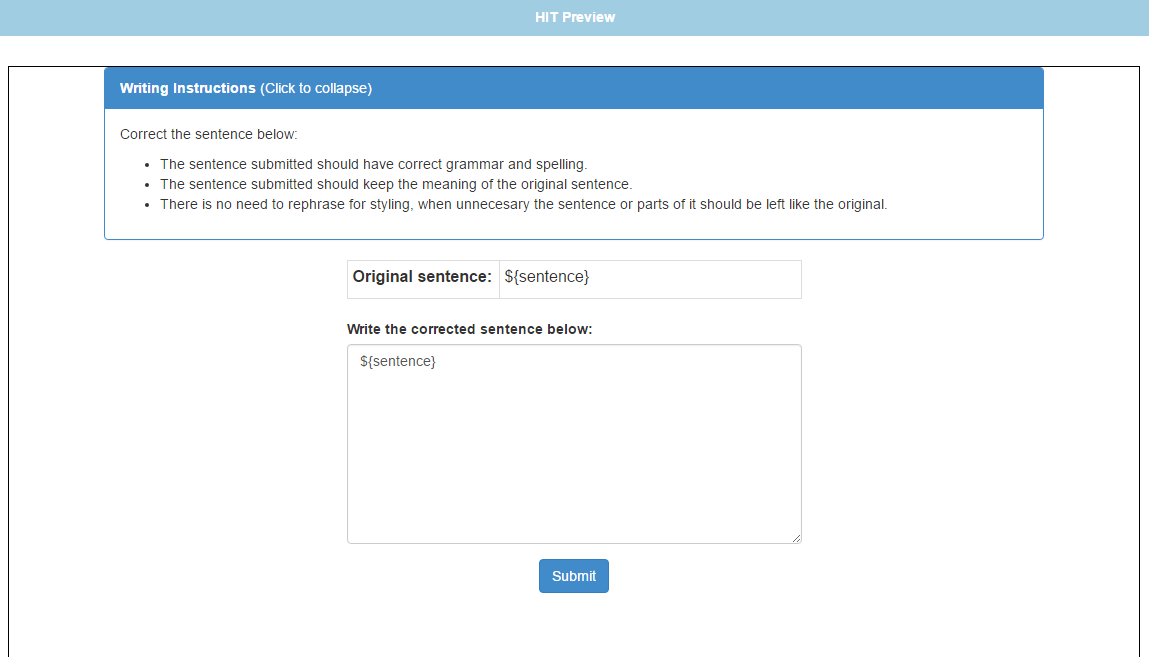
\includegraphics[width=0.9\columnwidth]{correction_task}
	\caption{Template for a grammatical error correction annotation task} 
\end{figure}
\FloatBarrier


\section{Additional figures}
\subsection{Validity}\label{ap:validity_judgements}
\begin{figure}[h!]
	\vspace{-.3cm}
	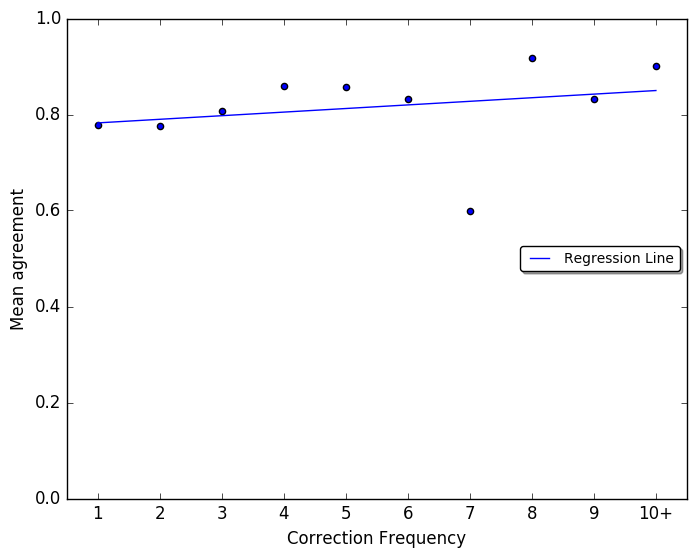
\includegraphics[width=0.9\columnwidth]{IAA_confirmation_frequency}
	\caption{The mean frequency ($y$-axis) in which a correction that was produced
		a given number of times ($x$-axis), was judged to be valid.
		\label{fig:validity_judgements}}
	\vspace{-0.3cm}
\end{figure}
\FloatBarrier

\section{Accuracy - Poisson Binomial Distribution}\label{ap:poibin}
The analytic tools we have developed support the computation of the entire distribution of the accuracy, and not only its expected values. From the Equation 
	
	\begin{myequation}
		Acc\left(C;X,Y\right) = \frac{1}{N} \sum_{i=1}^N \mathds{1}_{C(x_i) \in Y_i}.
	\end{myequation}
	
\noindent
 we see that Accuracy has a Poisson Binominal distribution (i.e., it is a sum of independent Bernoulli variables with different success probabilities), whose success probabilities are $P_{y,Y \sim \mathcal{D}_i}(y \in Y)$, which can be computed, as before, using our estimate for $\mathcal{D}_i$. Estimating the density function allows for the straightforward definition of significance tests for the measure, and can be performed efficiently \cite{hong2013computing}. An implementation of this and other methods for efficiently computing and approximating Poisson Binomial Distributions and the estimated density functions will be released upon publication.

\section{Type conservatism and prevalence}\label{ap:types}

\begin{table}[]
	\npdecimalsign{.}
	\nprounddigits{3}
	\centering
	\resizebox{0.3\textwidth}{!}{%
		\begin{tabular}{@{}ln{5}{2}@{}}
			\toprule
			\multicolumn{1}{c}{TYPE}       & \multicolumn{1}{c}{CHANGE}       \\ \midrule
			CONTR      & 0.9705882353 \\
			NOUN:NUM   & 0.9545454545 \\
			ORTH       & 0.8925       \\
			ADJ:FORM   & 0.8101265823 \\
			NOUN:INFL  & 0.7125       \\
			DET        & 0.6724801812 \\
			VERB:SVA   & 0.6434231379 \\
			MORPH      & 0.6150712831 \\
			VERB:FORM  & 0.5384615385 \\
			SPELL      & 0.5373737374 \\
			VERB:INFL  & 0.5          \\
			ADJ        & 0.4596273292 \\
			CONJ       & 0.4303797468 \\
			ADV        & 0.416091954  \\
			PREP       & 0.3343130051 \\
			WO         & 0.3148148148 \\
			NOUN:POSS  & 0.2904564315 \\
			VERB:TENSE & 0.2887673956 \\
			NOUN       & 0.2823240589 \\
			PART       & 0.268        \\
			PRON       & 0.2391033624 \\
			PUNCT      & 0.2012539185 \\
			OTHER      & 0.1736497941 \\
			VERB       & 0.1509009009 \\ \bottomrule
		\end{tabular}%
	}
	\caption{Number of mean corrections of systems divided by the number of corrections by references on NUCLE dataset\cite{dahlmeier2012better}. Data is based on \citet{bryant-felice-briscoe:2017:Long}.}
\end{table}
\FloatBarrier

\section{SARI with Multiple references}\label{ap:sari-assum}
Most RBMs define their multi-reference score to be the maximum score the
output attains against any single one reference.
SARI takes a different approach and combines multiple references to yield its score, 
possibly in order to compensate for the necessarily limited coverage of the available
references. This yields non-monotonic behavior of SARI with respect to increasing
the number of references, which makes the biases incurred by low coverage less predictable,
but not less significant.
For instance, a set of diverse set of references would span a large space of possible
combinations, making SARI more permissive. A set of references of the same size, which only differ little
from one another would yield a more conservative SARI score.

%If so, reference tendencies and distribution, are all the more relevant -- 
%gold standard is practically an aggregation of references and not individual one. Albeit agreeable assumption, the gold standard as reflected in a translation that achieves full SARI score is yet far from agreeable.
SARI is defined as the average of 3 scores, based on how well the system output kept the words it should keep,
deleted the words it should delete, and added the words it should add (all with respect to the reference).
Each of these scores behaves differently when increasing the number of references.
For a perfect recall for addition can only be obtained if all additions suggested by any reference are added. For a perfect precision for addition all additions should be found in at least one reference, acting similar to max operation. For a perfect precision on keeping all the references should keep all agree on keeping everything the system kept, and as we showed reference don't tend to agree on it. For a perfect recall the system should everything that at least one of the references chose to keep. Note, that the two terms together mean that for a perfect keep score a necessary condition is that all \textbf{references} should agree on what to keep. A perfect precision of deletion acts similarly to the one over keeping, but being precision oriented SARI ignores the deletion recall. Thus, a perfect deletion would be one to delete only words, and at least one, that all references agree on.
%For instance, a perfect recall for addition can only be obtained if all additions suggested by any reference are added, 
%it is practically impossible to get full score on the other types of changes, the gained score is weighted by the amount of references agreeing on it, and as we showed, references don't tend to.


\section{Reference Crowdsourcing for Simplification}\label{ap:simp-rerank}
In order to perform our simplification experiments, 
we collected additional references for sentences from the corpus presented in \newcite{Xu-EtAl:2016:TACL}, using Amazon
Mechanical Turk with similar annotation guidelines to those used by Xu et al. 
Overall we collect 50 references for 45, and 100 and 150 references for two more sentences.
The latter two have 70 and 126 references that occur only once and none reoccurring more than 6 times, 
supporting the claim that the size of the space of valid references for TS is huge.
Standard worker rejection techniques were used, but no worker had to be rejected.

\begin{figure}[h!]
	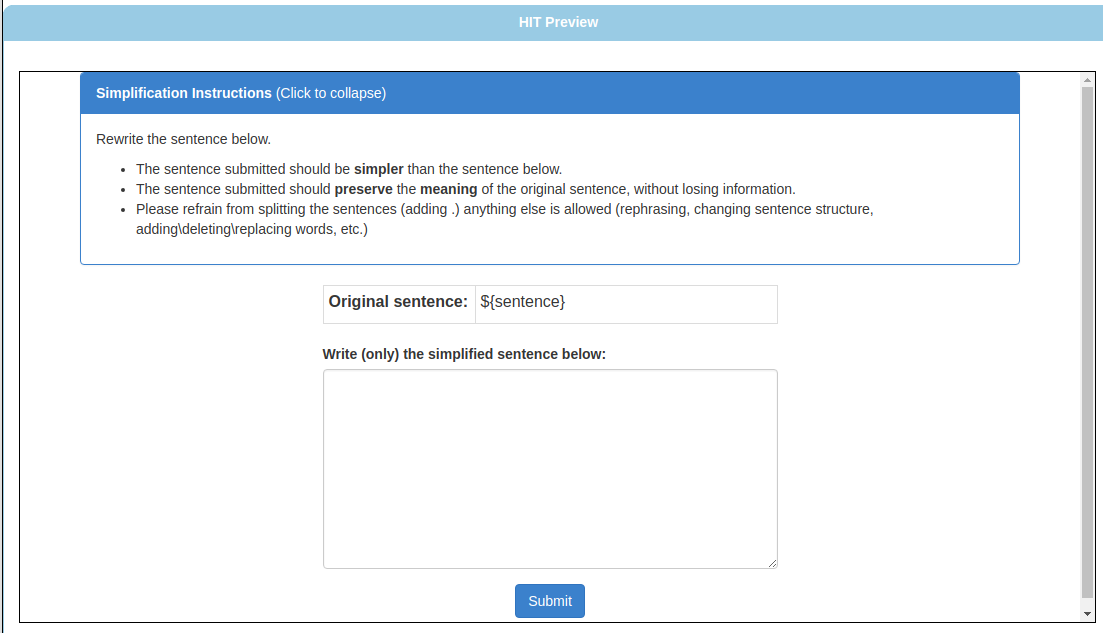
\includegraphics[width=0.9\columnwidth]{simplification_task}
	\caption{Template for a simplification annotation task} 
\end{figure}
\FloatBarrier
\subsection{Simplification reranking}
\begin{figure}[h!]
	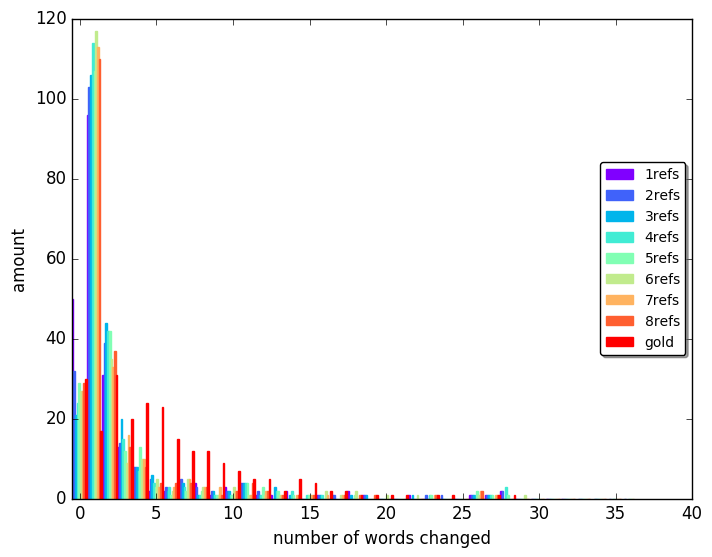
\includegraphics[width=0.9\columnwidth]{nisioi_max_words_differences_hist}
	\caption{Reranking results with \newcite{nisioi2017exploring} and MAX-SARI}
\end{figure}
\begin{figure}[h!]
	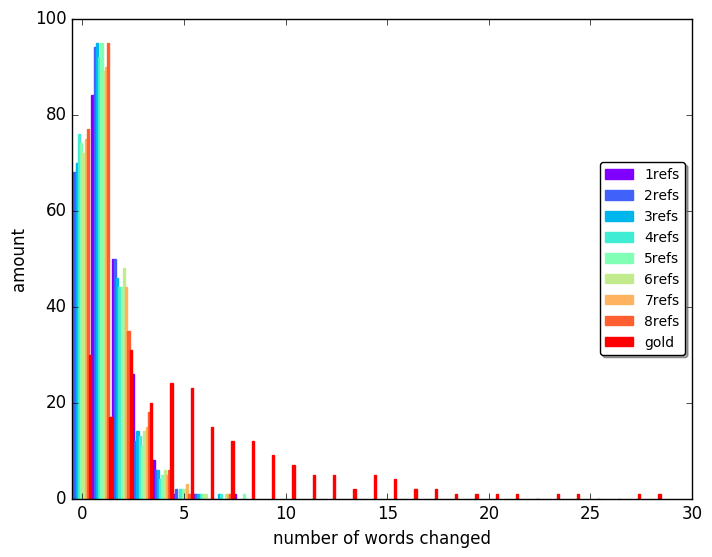
\includegraphics[width=0.9\columnwidth]{moses_sari_words_differences_hist}
	\caption{Reranking results with Moses and SARI}
	
\end{figure}
\begin{figure}[h!]
	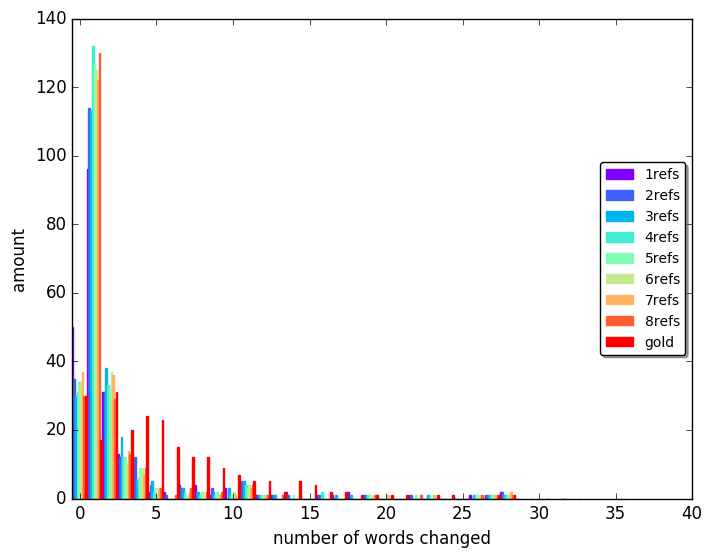
\includegraphics[width=0.9\columnwidth]{nisioi_sari_words_differences_hist}
	\caption{Reranking results with \newcite{nisioi2017exploring} and SARI}
	
\end{figure}
\begin{figure}[h!]
	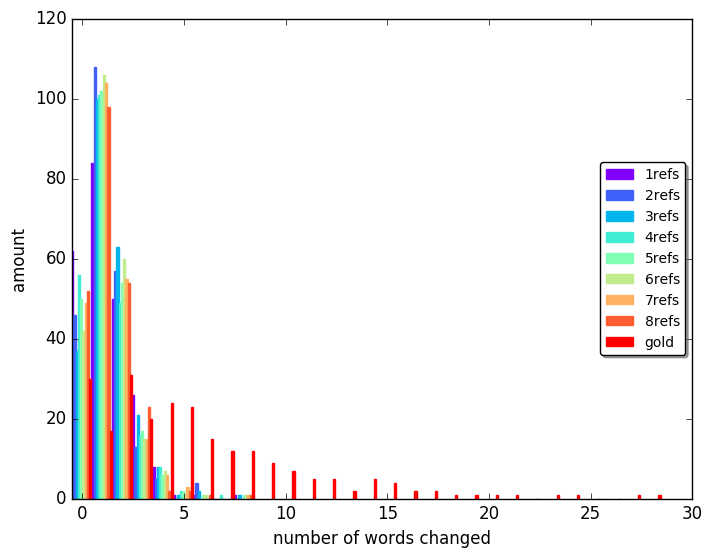
\includegraphics[width=0.9\columnwidth]{moses_max_words_differences_hist}
	\caption{Reranking results with Moses and MAX-SARI}
	
\end{figure}
\FloatBarrier
\com{
	\section{Annotated paragraphs}
	\begin{table}[hb]
		\centering
		\begin{tabular}{lll}
			Annotator-id & NUCLE-id & type      \\
			1         & 2  & corrected \\
			2         & 2  & corrected \\
			1         & 2  & learner   \\
			2         & 2  & learner   \\
			1         & 3  & corrected \\
			2         & 3  & corrected \\
			1         & 3  & learner   \\
			2         & 3  & learner   \\
			1         & 5  & corrected \\
			2         & 5  & corrected \\
			1         & 5  & learner   \\
			2         & 5  & learner   \\
			1         & 6  & learner   \\
			2         & 6  & learner   \\
			2         & 7  & corrected \\
			2         & 7  & learner   \\
			1         & 8  & corrected \\
			1         & 8  & learner   \\
			1         & 10 & corrected \\
			1         & 10 & learner  
		\end{tabular}
		\caption{The list of paragraphs annotated, showing which annotator annotated it, which type of language is used in it and the corresponding id in the NUCLE corpus. Note that parallel paragraphs have the same id.\label{tab:annotated-paragraphs}}
	\end{table}
}
\FloatBarrier



\bibliographystyle{acl_natbib}
\bibliography{propose}
\end{document}
